\documentclass{article}
\usepackage{titling}
\usepackage[T1]{fontenc}
\usepackage[polish]{babel}
\usepackage[OT4]{fontenc} 
% Margins in document
\usepackage[left=1.5cm, right=1.5cm, top=3cm]{geometry}

% Avoid  colons before tables' empty captions and change caption
\usepackage{caption}
\captionsetup[table]{name=Tab.}
\captionsetup[figure]{name=Rys.}
\usepackage{hyperref}

% Don't know why, it starts from 2
\addtocounter{table}{-1}

% Rename tables' suffix
\renewcommand{\tablename}{Tab.}

% Graphicx setup
\usepackage{graphicx}
\graphicspath{{grafiki/}{../grafiki/}}

% No separator between items
\usepackage{enumitem}
\setlist{nolistsep}

% Pagebreak before every \section
\let\oldsection\section
\renewcommand\section{\clearpage\oldsection}

% Vhistory setup
\usepackage[owncaptions]{vhistory}
\renewcommand{\vhhistoryname}{Historia zmian}
\renewcommand{\vhversionname}{Wersja}
\renewcommand{\vhdatename}{Data}
\renewcommand{\vhauthorname}{Autor(zy)}
\renewcommand{\vhchangename}{Zmiany}

% Bigger padding in tabulars
\usepackage{array}
\setlength\extrarowheight{3pt}

% Itemize in tabulars (avoid big margins with minipage)
\newcommand{\tabbeditemize}[1]{
	\begin{minipage}[t]{0.4\textwidth}
		\begin{itemize}[topsep=0mm,partopsep=0mm,leftmargin=4mm]
			#1
		\end{itemize}
\end{minipage}}

% Code command
\usepackage{xcolor}
\definecolor{light-gray}{gray}{1}
\newcommand{\code}[1]{\colorbox{light-gray}{\texttt{#1}}}

% Modulename command
\newcommand{\modulename}[1]{\textit{#1}}

% Listings setup
\usepackage{listings}
\definecolor{codegreen}{rgb}{0,0.6,0}
\definecolor{codegray}{rgb}{0.5,0.5,0.5}
\definecolor{codepurple}{rgb}{0.58,0,0.82}
\definecolor{backcolour}{rgb}{0.95,0.95,0.92}
\lstdefinestyle{mystyle}{
	backgroundcolor=\color{backcolour},   
	commentstyle=\color{codegreen},
	keywordstyle=\color{magenta},
	numberstyle=\tiny\color{codegray},
	stringstyle=\color{codepurple},
	basicstyle=\ttfamily\footnotesize,
	breakatwhitespace=false,         
	breaklines=true,                 
	captionpos=b,                    
	keepspaces=true,                 
	numbers=left,                    
	numbersep=5pt,                  
	showspaces=false,                
	showstringspaces=false,
	showtabs=false,                  
	tabsize=2
}
\lstset{style=mystyle}

% DOCUMENT
\title{
	Wizualizacja drzewa stanów algorytmu UCT \\
	\large Dokumentacja powykonawcza}

\author{Patryk Fijałkowski \\ Grzegorz Kacprowicz}
\begin{document}
\begin{titlingpage}
	\maketitle
	\vspace{3cm}
	\begin{abstract}
		Poniższy dokument zawiera dokumentację powykonawczą projektu, którym było stworzenie aplikacji pozwalającej na wizualizację drzewa stanów algorytmu UCT. Ma ona w zamyśle pozwalać na oglądanie i dokładną analizę rozgrywki z komputerem podczas grania w jedną z dwóch gier planszowych. Dokument przeprowadza czytelnika przez instrukcję poprawnego uruchomienia programu oraz opis funkcjonalności połączony z instrukcją użytkowania. Będzie on zawierał również opis interfejsu użytkownika, dokładnie opisujący najistotniejsze okna aplikacji. Dokument pozwala także zaznajomić się z architekturą programu oraz opisem i schematami modułów aplikacji - zaczynając od tego odpowiedzialnego za wizualizację. Pierwszy moduł, będący najistotniejszym, będzie opierał się na usprawnionej wersji algorytmu Walkera. Opisane są również moduły odpowiedzialne za logikę zaimplementowanych gier, implementację algorytmu oraz serializowanie generowanych drzew wraz ze schematami serializacji. \modulename{Aplikacja główna}, czyli ostatni opisywany moduł, jest modułem służącym do prezentacji działania poprzednich modułów. Ostatni rozdział dokumentu opisuje i uzasadnia technologie wybrane do stworzenia aplikacji.
	\end{abstract}
\end{titlingpage}

\begin{versionhistory}
	\vhEntry{1.0}{14.12.2019}{PF|GK}{stworzenie szkicu dokumentu}
	\vhEntry{1.1}{17.12.2019}{PF|GK}{stworzenie pierwszej wersji dokumentu}
\end{versionhistory}
\tableofcontents
	
\section{Instrukcja uruchamiania}
Aplikacja została napisana w języku \textit{Python}, zatem klient powinien zainstalować jego interpreter, który może znaleźć na stronie: \url{https://www.python.org/downloads/}. Wymagana wersja to Python 3.7.2 lub nowsza.\\
Do tak ściągniętego interpretera załączony jest również \textit{pip} - menedżer pakietów Python. Za jego pomocą należy pobrać niezbędny pakiet. Przed pobraniem pakietów zalecane jest uaktualnienie menedżera następującą komendą:
\begin{itemize}
	\item na Windowsie:
	\begin{lstlisting}
	python -m pip install -U pip\end{lstlisting}
	\item na Linuxie:
	\begin{lstlisting}
	pip install -U pip\end{lstlisting}
\end{itemize}
Następnie, należy uruchomić następującą komendę w konsoli, aby pobrać pakiet PyQt5, o którym więcej będzie w ostatnim rozdziale dokumentu:
\begin{lstlisting}
pip install PyQt5
\end{lstlisting}
Ze względu na fakt, iż Python jest językiem interpretowanym, program również należy uruchomić \underline{z poziomu konsoli}. 
Należy zatem przejść do katalogu \textbf{/uct-visualization/src/main\_application} i wpisać komendę:
\begin{lstlisting}
python main_application_window.py
\end{lstlisting}
lub uruchomić program z głównego katalogu aplikacji \textbf{/uct-visualization}:
\begin{lstlisting}
python /uct-visualization/src/main_application/main_application_window.py
\end{lstlisting}
Po uruchomieniu powinniśmy zobaczyć główne okno aplikacji o nazwie \textit{UCT Visualizer}.

\section{Poradnik użytkowania i opis funkcjonalności}
Dla wygodnej interakcji użytkownika z programem przygotowany został specjalny interfejs graficzny. Możemy wyróżnić trzy główne okna.
\subsection{Okno startowe aplikacji}
Jest to główne okno programu, w którym użytkownik może wybrać, czy chce zagrać w grę, czy wczytać i obejrzeć przygotowane wcześniej pliki drzew. Okno prezentuje się następująco:
\begin{center}
	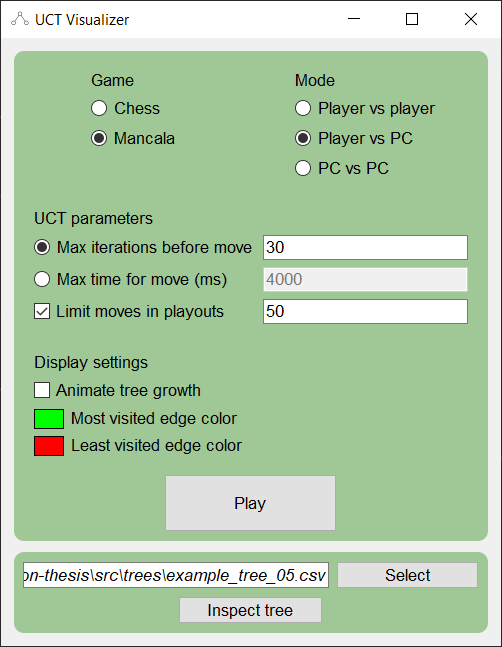
\includegraphics[width=0.45\textwidth]{main-app-window}
\end{center}
Dostępne funkcje:\\
\begin{enumerate}
	\item Wybór jednej z dwóch gier:
	\subitem $\bullet$ mancala
	\subitem $\bullet$ szachy.\\
	\item Wybór jednego z trzech trybów gry:
	\subitem $\bullet$ \textit{gracz vs PC} - po wykonanym ruchu gracza algorytm oblicza ruch komputera i wykonuje go
	\subitem $\bullet$ \textit{PC vs PC }- użytkownik decyduje, kiedy mają wykonać się ruchy komputera
	\subitem $\bullet$ \textit{gracz vs gracz} - rozgrywka dwóch graczy, co wiąże się z brakiem wizualizacji.\\
	\item Ustawienie parametrów ruchu algorytmu UCT:
	\subitem $\bullet$ ilość wykonanych iteracji - im więcej ich będzie, tym więcej razy powtórzone będą kroki symulacji kolejnego ruchu przez komputer, co przekłada się na jego większą dokładność i trafność. Minusem jest większy czas oczekiwania na wykonaniu ruchu. (przedział: 1-10000)
	\subitem $\bullet$ maksymalny czas na wykonanie ruchu przez komputer - opcja alternatywna dla powyższej. Zamiast podawać odgórnie ilość iteracji, użytkownik może podać czas, w jakim komputer będzie wyznaczał ruch. Po upłynięciu czasu ostatnia symulacja jest dogrywana. (przedział: 1000ms - 30000ms).\\
	\item Ucięcie iteracji po przekroczeniu arbitralnie ustalonej liczby ruchów danego ``playoutu'' (symulacji rozgrywki w obrębie iteracji). Opcja może być włączona lub wyłączona. Dla tego drugiego przypadku gra kończy się tylko wtedy, gdy symulacja gry zakończy się w naturalny sposób.\\
	\item Włączenie animacji rozrostu drzewa - pozwala obserwować jak zmieniało się drzewo w trakcie symulacji ruchu - drzewo wyświetlane jest po każdej iteracji algorytmu. W przypadku wybrania opcji maksymalnego czasu na wykonanie ruchu przez komputer ta opcja uwzględni również czas rysowania wszystkich drzew, co wiąże się ze stratą wydajności algorytmu.\\
	\item Wybór kolorów krawędzi - dla ruchów najczęściej i najrzadziej odwiedzanych przez algorytm. Kolory pozostałych krawędzi będą gradientami podanych kolorów - dla powyższego przykłądowego okna, krawędzie częściej odwiedzanych węzłów będą bardziej zielone i mniej czerwone.\\
	\item Wybór drzew do przeglądu - po kliknięciu przycisku \textit{Select} otwiera się dodatkowe okno, które prosi użytkownika o wybranie pliku bądź zestawu plików drzew do analizy. Przyjmowane będą pliki w formacie .csv i binarnym (.tree), w ktorych dane zapisane będą według ustalonego schematu. Zakładamy poprawność wczytywanych plików. W polu tekstowym wyświetli się wówczas ścieżka do wczytanego pliku lub liczba plików w przypadku wczytania ich większej liczby.\\
\end{enumerate}
Aby rozpocząć rozgrywkę, należy nacisnąć przycisk \textit{Play}. Aby wizualizować wczytane drzewa - \textit{Inspect tree}.
\subsection{Okno podglądu drzewa}
Okno to umożliwia wizualizację drzew z wczytanych plików oraz sprawne poruszanie się po niej, wraz z możliwością wyświetlania statystyk poszczególnych węzłów:
\begin{center}
	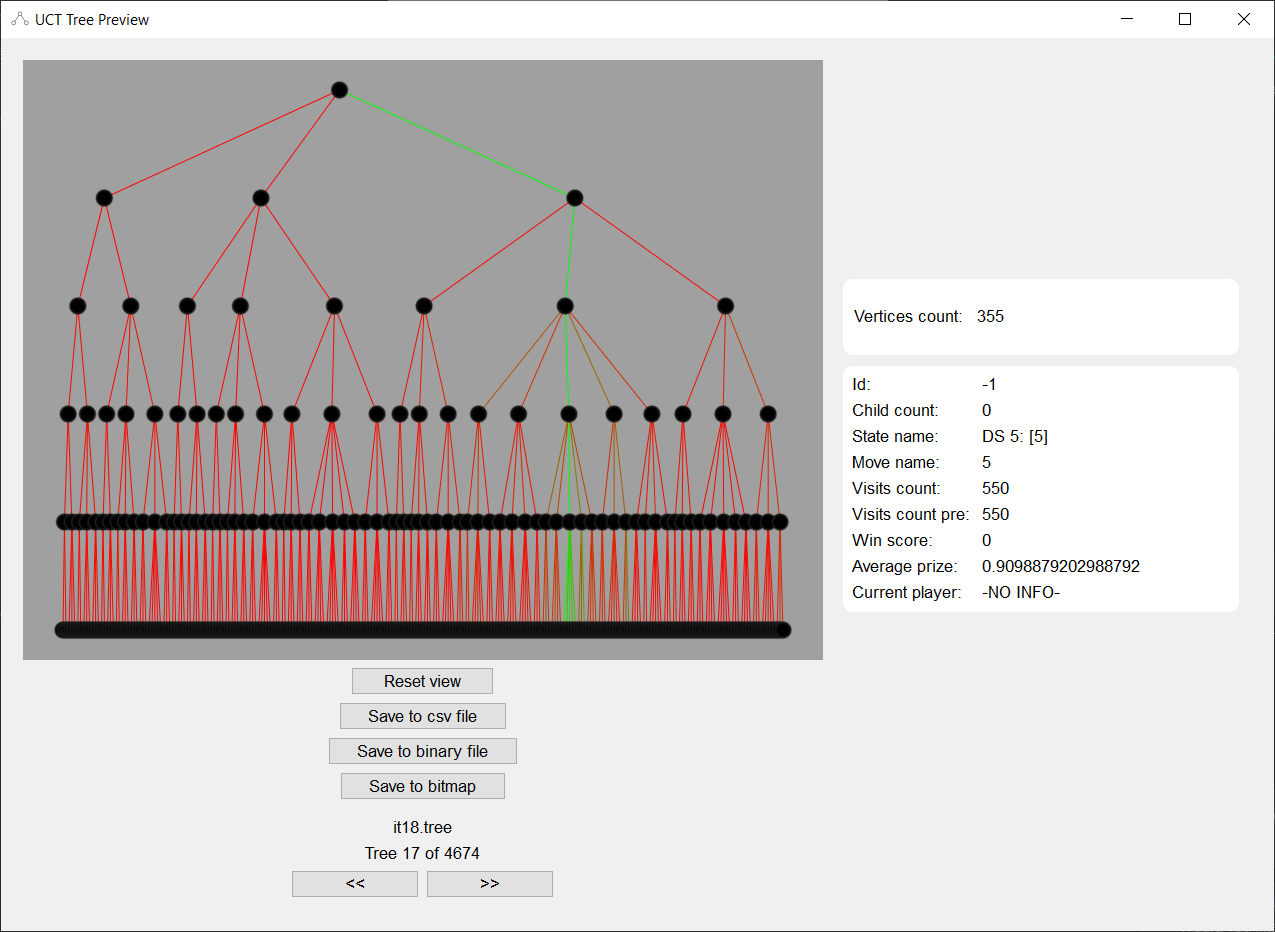
\includegraphics[width=0.8\textwidth]{tree-window}
\end{center}
Dostępne funkcje:\\
\begin{enumerate}
	\item Przybliżanie i oddalanie drzewa za pomocą scrolla. Kursor musi znajdować się nad częścią okna, gdzie wyświetlane jest drzewo.\\
	\item Przesuwanie drzewa - należy przytrzymać prawy przycisk myszy i poruszać myszką.\\
	\item Wyświetlenie statystyk węzła - należy kliknąć lewym przyciskiem myszy na dany węzeł. Po wybraniu węzła, po prawej stronie wyświetlają się jego statystyki:
	\subitem $\bullet$ ilość wszystkich wierzchołków drzewa
	\subitem $\bullet$ identyfikator węzłą
	\subitem $\bullet$ ilość węzłów-dzieci
	\subitem $\bullet$ nazwa stanu
	\subitem $\bullet$ nazwa ruchu
	\subitem $\bullet$ liczba odwiedzin węzła przez algorytm
	\subitem $\bullet$ suma wszystkich wygranych (łącznie wyniki poztywne i negatywne)
	\subitem $\bullet$ średnia wygrana - suma wygranych $\div$ ilość odwiedzin. Wartość z przedziału $[0, 1]$
	\subitem $\bullet$ numer gracza, który wykonał ruch dla danego węzła (1 lub 2).\\
	\item Wyśrodkowanie drzewa - resetuje stopień przybliżenie i przesunięcia.\\
	\item Zapis drzewa:
	\subitem $\bullet$ w formacie .csv
	\subitem $\bullet$ w formacie binarnym (.tree)
	\subitem $\bullet$ jako bitmapa (.png).\\
	\item Zmiana drzewa w sekwencji - możemy robić to za pomocą przycisków \textit{<<} i \textit{>>} na ekranie lub za pomocą strzałek na klawiaturze. Wyświetlana jest nazwa aktualnie przeglądanego pliku oraz to, którym jest on plikiem z kolei.\\
\end{enumerate}
Zamknięcie tego okna nie kończy programu - okno menu głównego jest ciągle aktywne i może być wykorzystane ponownie.

\subsection{Okno gry i wizualizacji}
Jest to połączenie gry oraz okna podglądu drzewa opisanego powyżej. Znajduje się tu interfejs graficzny toczącej się gry, w którą może ingerować użytkownik i wykonywać swoje ruchy. W górnej części znajduje się pasek postępu, który odzwierciedla ilość wykonanych przez algorytm iteracji podczas wyznaczania następnego ruchu. Po jego wyznaczeniu w środkowej częsci okna ukazuje się wygenerowane drzewo. Jeżeli użytkownik włączył opcję animacji drzew w menu głównym, dodatkowo po każdej iteracji będzie mógł on oglądać rozrost drzewa.\\
\begin{center}
	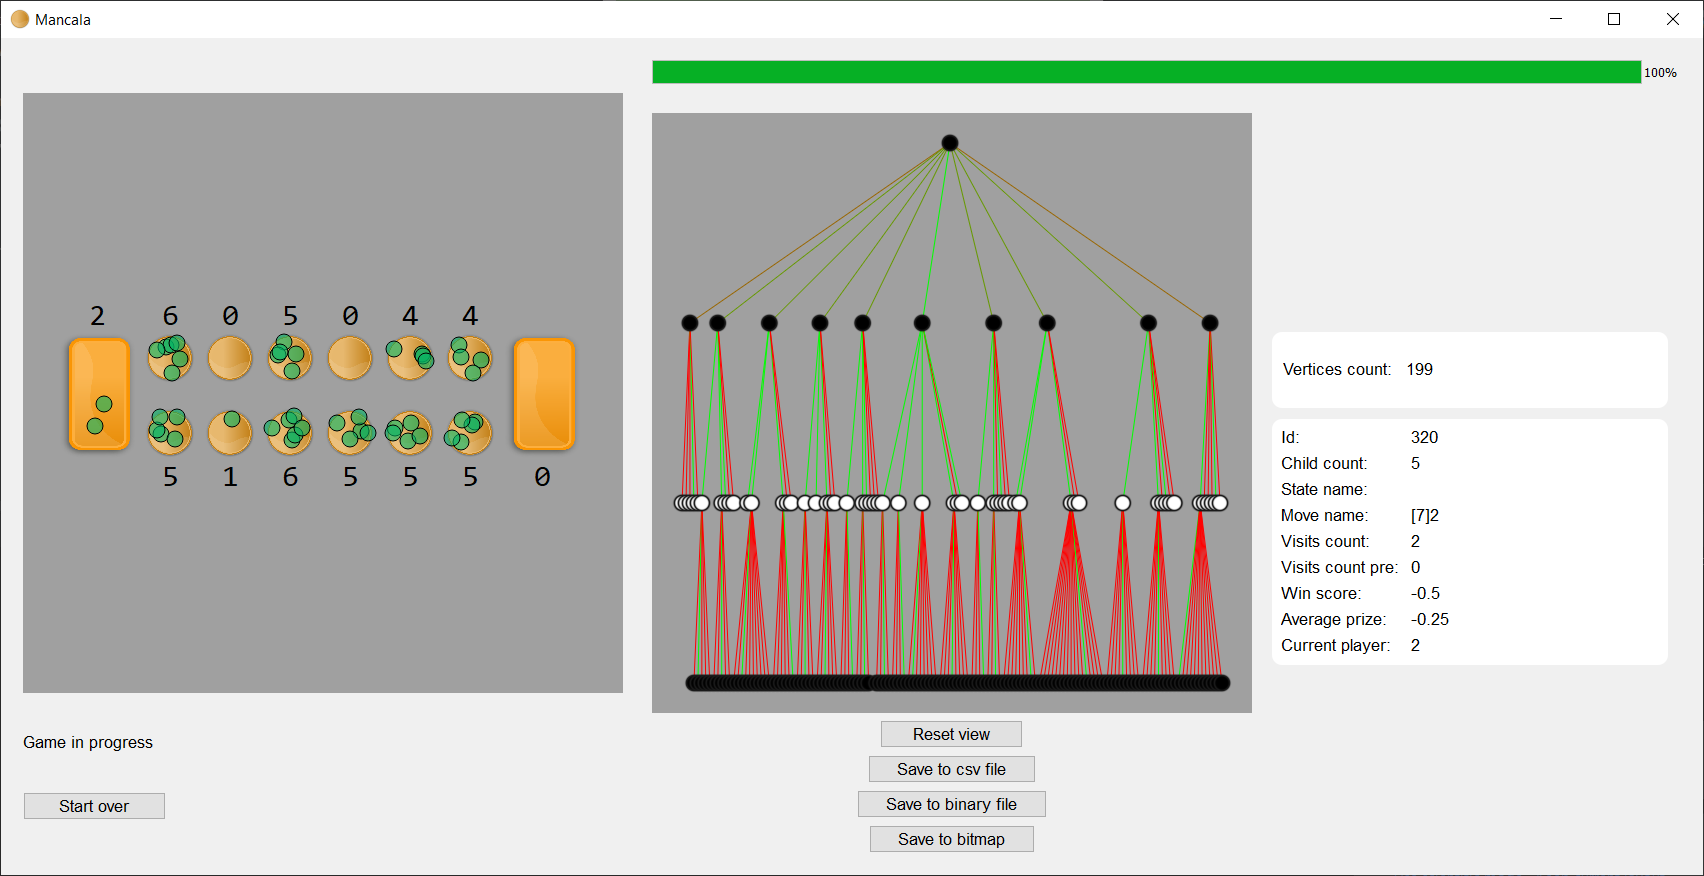
\includegraphics[width=\textwidth]{game-window}
\end{center}
Dostępne funkcje:\\
\begin{enumerate}
	\item Wszystkie funkcje dostępne w oknie podglądu drzewa poza sekwencjami.\\
	\item Wykonanie ruchu z pomocą GUI gry, np. kliknięcie danego pola w szachach lub dołka w mancali. Nie dotyczy trybu \textit{gracz vs PC}. Po zakończonej rozgrywce napis \textit{Game in progress} pod polem gry zmienia wartość i oznajmia użytkownikowi, która strona wygrała (lub czy jest remis).\\
	\item Rozegranie gry od nowa - kliknięcie przycisku \textit{Start over}.\\
	\item Wykonanie następnego ruchu za pomocą przycisku - tylko w trybie \textit{PC vs PC}. Pozwala na spowodowanie postępu w symulacji rozgrywki komputera z samym sobą. Ruchy za pomocą GUI są wówczas zablokowane.\\
\end{enumerate}
Zamknięcie tego okna również nie kończy programu - okno menu głównego jest ciągle aktywne i może być wykorzystane ponownie.

\section{Architektura systemu}
Aplikacja jest podzielona na pięć oddzielnych modułów: \modulename{algorytm}, \modulename{serializacja}, \modulename{wizualizacja}, \modulename{gry}, które będą funkcjonować w obrębie nadrzędnego modułu - \modulename{aplikacji głównej}. 


\subsection{Diagram klas głównych komponentów}

\noindent Rysunek \ref{rys:umldiagrammain} ukazuje diagram klas najważniejszych komponentów związanych z modułami \modulename{Algorytm}, \modulename{Wizualizacja} i \modulename{Serializacja}.

\begin{figure}[h]
	\centering
	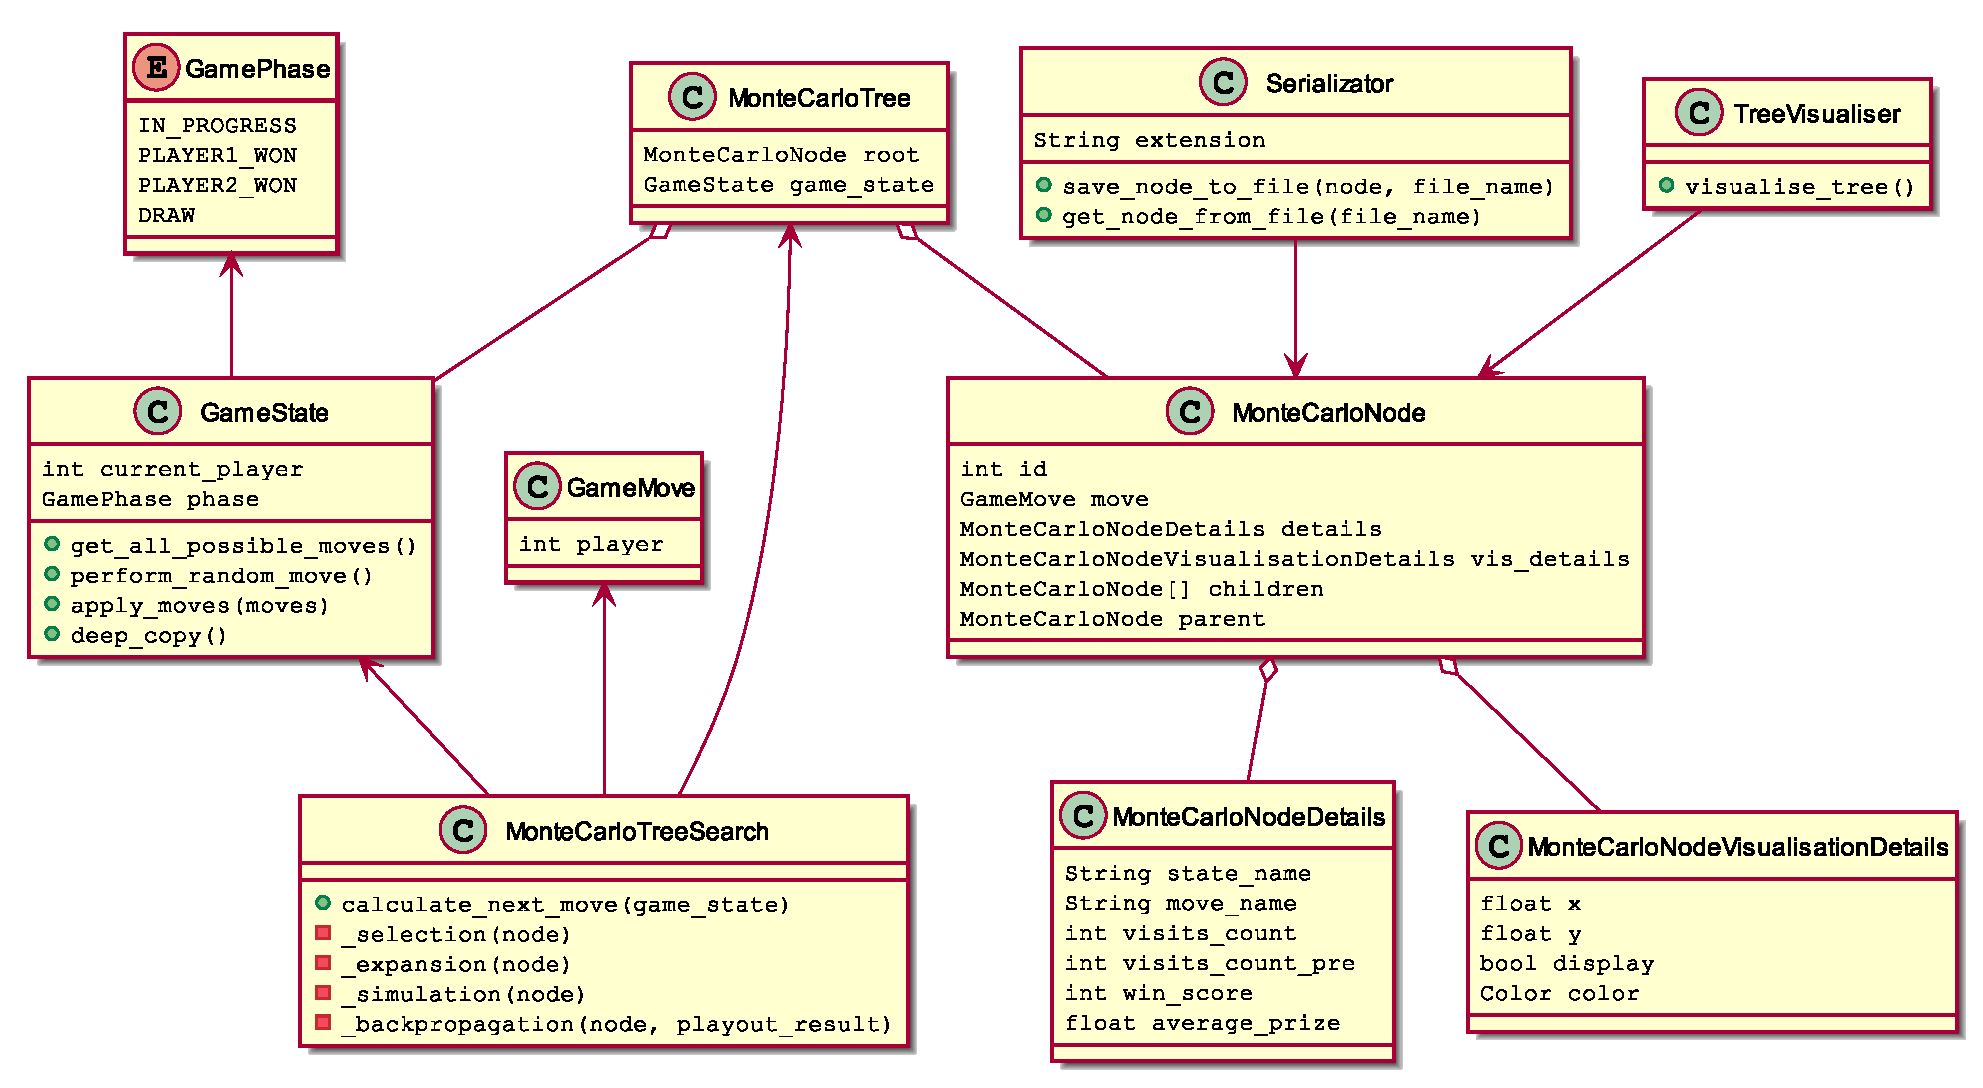
\includegraphics[width=0.9\textwidth]{umldiagram}
	\caption{Diagram klas głównych komponentów}
	\label{rys:umldiagrammain}
\end{figure}
\noindent Zgodnie z diagramem, klasy \code{MonteCarloTreeSearch}, \code{TreeVisualiser} oraz \code{Serializator} są pośrednio lub bezpośrednie zależne od klasy \code{MonteCarloNode}, opisującej wierzchołek w drzewie. Jest to część wspólna modułów \modulename{Algorytm}, \modulename{Wizualizacja} i \modulename{Serializacja}. Klasa \code{MonteCarloNode} przechowuje referencję do swojego rodzica oraz wierzchołków potomnych, aby zachować rekurencyjną strukturę drzewa.\\

\noindent Metoda \code{calculate\textunderscore next\textunderscore move} klasy \code{MonteCarloTreeSearch} odpowiada za wykonanie kolejnych iteracji algorytmu. Algorytm zapisuje informacje o rozgrywanych playoutach w polach klasy \code{MonteCarloNodeDetails} analizowanych wierzchołków. Ruch oraz stan analizowanej gry są opisane odpowiednio przez klasy \code{GameMove} i \code{GameState}. Implementacja metod tych klas daje możliwość łatwego rozszerzenia aplikacji o inne gry. Istotny z punktu widzenia konstrukcji drzewa jest stan rozgrywki, który opisują pola typu wyliczeniowego \code{GamePhase}.

\clearpage

\noindent \code{TreeVisualiser} jest głównym komponentem modułu \modulename{Wizualizacja}. Jego odpowiedzialnością jest wyznaczenie układu wierzchołków drzewa na płaszczyźnie oraz wyświetlenie wygenerowanej wizualizacji. Szczegóły związane z rysowaniem każdego wierzchołka, takie jak jego współrzędne czy kolor, zawarte są w polach klasy \code{MonteCarloVisualisationDetails}.\\

\noindent \code{Serializator} jest klasą opisującą funkcjonalności, które mają udostępnić właściwe implementacje serializatorów, czyli serializowanie drzew do plików oraz deserializację z plików.


\subsection{Diagram stanów aplikacji}
\noindent Rysunek \ref{rys:statediagram} ukazuje diagram stanów aplikacji w przypadku rozgrywki w trybie \modulename{człowiek kontra maszyna}. 
\begin{figure}[h]
	\centering
	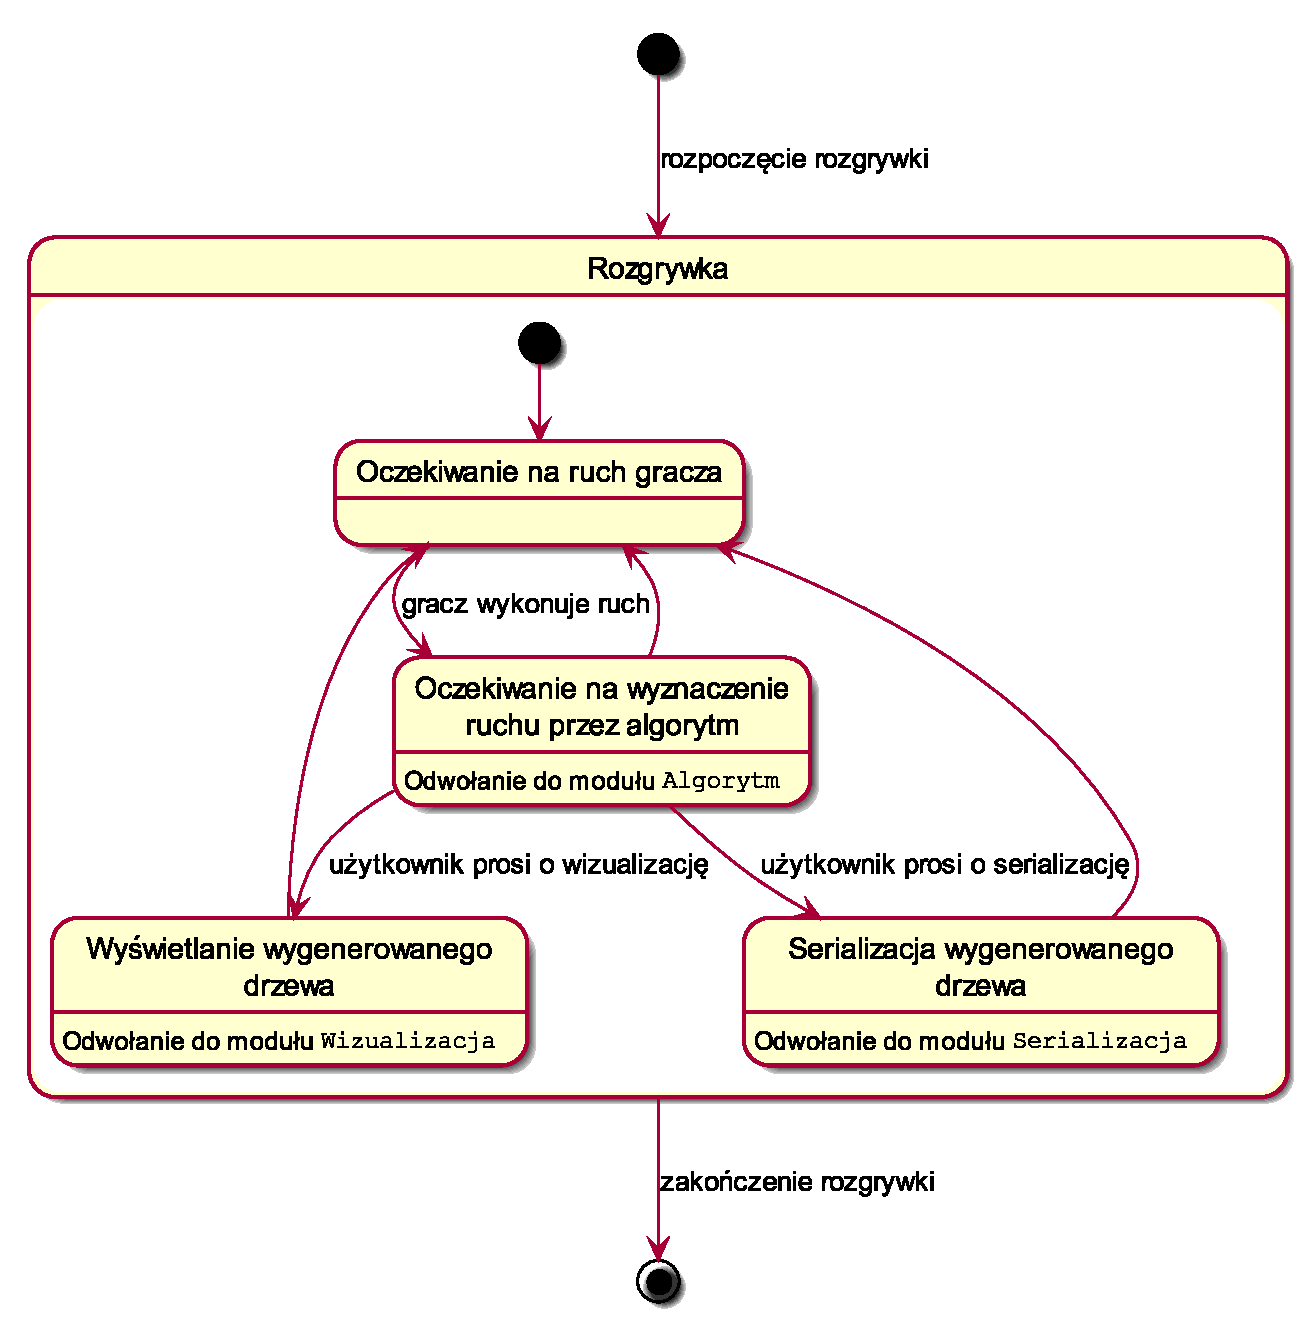
\includegraphics[width=0.7\textwidth]{statediagram}
	\caption{Diagram stanów aplikacji}
	\label{rys:statediagram}
\end{figure}

\noindent Zgodnie z diagramem, aplikacja po rozpoczęciu rozgrywki przechodzi do obszernego stanu \modulename{Rozgrywka}, zawierającego cztery wewnętrzne stany. Będac w stanie \modulename{Rozgrywka}, aplikacja może potencjalnie korzystać z każdego modułu aplikacji. \\

\noindent Istotna z punktu widzenia użytkownika jest możliwość serializowania wygenerowanego drzewa lub jego wizualizacja zaraz po ruchu wyznaczonym przez algorytm, co powoduje przejście aplikacji odpowiednio w stany \modulename{Serializacja wygenerowanego drzewa} oraz \modulename{Wyświetlanie wygenerowanego drzewa}.
\clearpage

\subsection{Diagram sekwencji rozgrywki}
Rysunek \ref{rys:sequencegame} ukazuje diagram sekwencji rozgrywki w trybie \modulename{człowiek kontra maszyna}.
\begin{figure}[h]
	\centering
	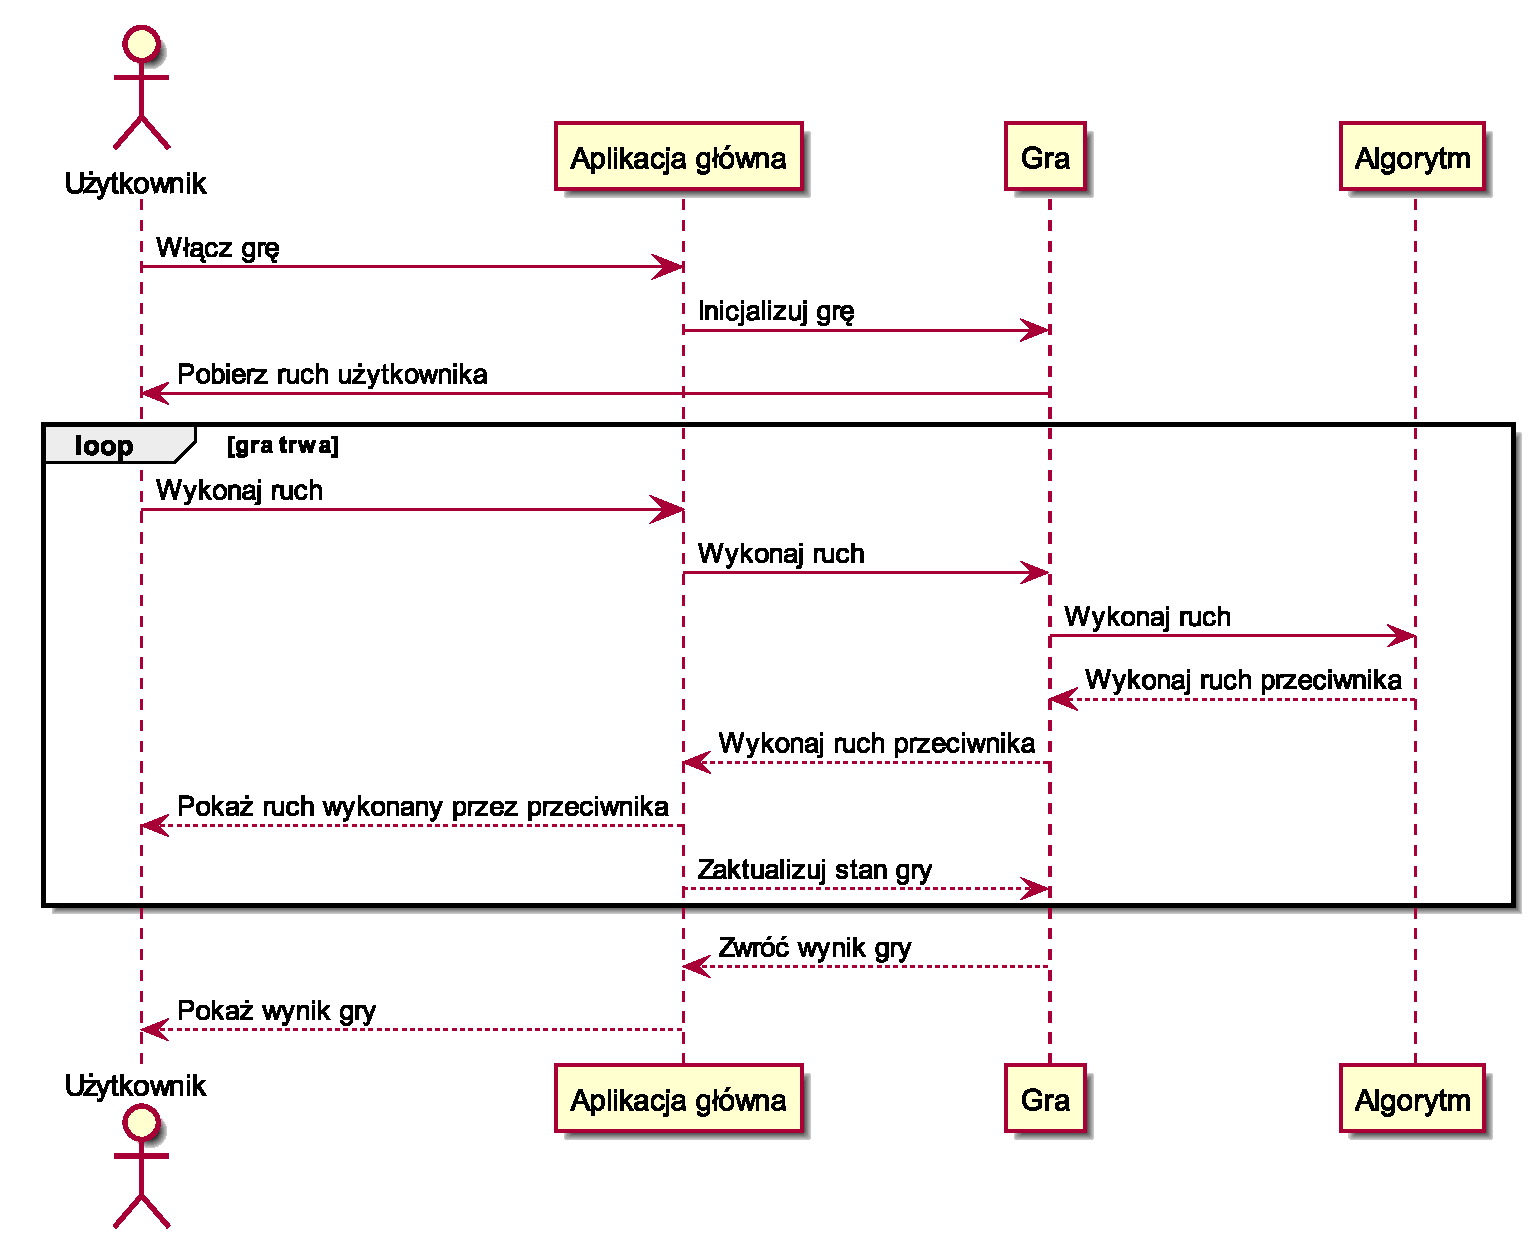
\includegraphics[width=0.8\textwidth]{play_with_pc_sequence}
	\caption{Diagram sekwencji rozgrywki}
	\label{rys:sequencegame}
\end{figure}

\noindent Istotne jest, jak w tej sytuacji komunikują się ze sobą moduły \modulename{Aplikacja główna}, \modulename{Gra} i \modulename{Algorytm}. Zgodnie z założeniami, \modulename{Aplikacja główna} jest interfejsem użytkownika do korzystania z pozostałych modułów.\\

\noindent Użytkownik końcowy za pomocą menu aplikacji głównej może ustawić parametry gry i następnie włączyć ją. Inicjalizowana jest wówczas rozgrywka w komponencie \textit{Gra}. Następnie, dopóki gra trwa i możliwe jest wykonanie ruchu, wykonywane są na zmianę ruchy gracza i PC - wymaga to komunikacji odpowiednio użytkownika z aplikacją główną, aplikacji głównej z grą i gry z modułem \modulename{Algorytm} (i vice versa). Po zakończeniu rozgrywki gra zwraca swój stan, który jest możliwy do zobaczenia przez użytkownika poprzez okno aplikacji głównej.\\

\noindent Diagram ukazuje, że w tym trybie każdy ruch gracza jest ściśle związany z odpowiedzią od modułu \modulename{Algorytm}, który pobiera stan rozgrywki z modułu \modulename{Gra}.

\clearpage
\subsection{Diagram sekwencji eksportu drzewa}
Rysunek \ref{rys:sequenceserialize} przedstawia proces współpracy różnych komponentów aplikacji w celu wyeksportowania wygenerowanego przez algorytm drzewa. Proces uruchamiania gry i wykonywania ruchów jest analogiczny do tego na rysunku \ref{rys:sequencegame}. 
\begin{figure}[h]
	\centering
	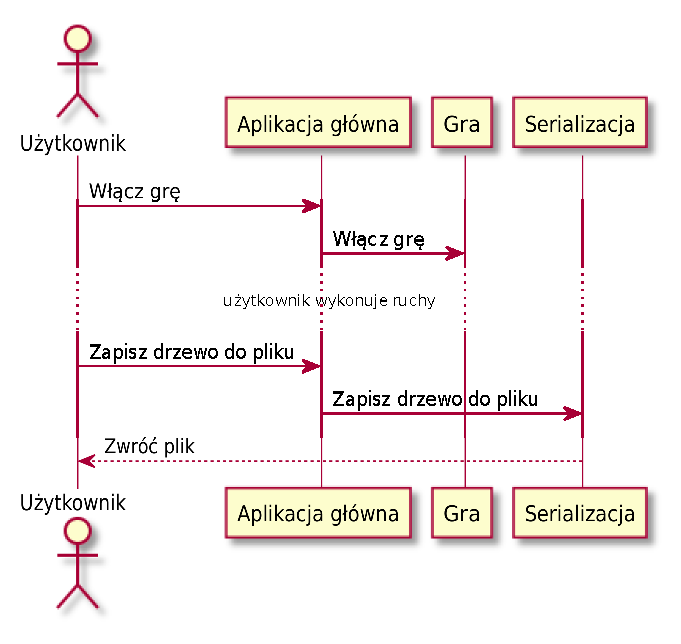
\includegraphics[width=0.6\textwidth]{serialize_sequence_simplified}
	\caption{Diagram sekwencji eksportu drzewa}
	\label{rys:sequenceserialize}
\end{figure}

\noindent Istotną cechą zaprojektowanego rozwiązania jest to, że gracz może wyeksportować drzewo w dowolnym momencie rozgrywki (po każdym ruchu przeciwnika). Żądanie takiej operacji przez użytkownika przesyłane jest do aplikacji głównej, która następnie komunikuje się z modułem odpowiedzialnym za serializację, który zapisuje drzewo do pliku. Plik drzewa zapisywany jest do specjalnego folderu na tego typu pliki i posiada datę wygenerowania.\\

\noindent Jest to diagram dla ustawienia \modulename{człowiek kontra maszyna}, jednak w przypadku \modulename{maszyna kontra maszyna} istnieje taka sama funkcjonalność i diagram byłby analogiczny.

\clearpage
\subsection{Diagram sekwencji wizualizacji}
Rysunek \ref{rys:sequencevisualise} przedstawia proces uruchamiania wizualizacji drzewa przez użytkownika jako współpracę poszczególnych komponentów aplikacji. Ponownie, proces uruchamiania gry i wykonywania ruchów wygląda tak jak na rysunku \ref{rys:sequencegame}. 
\begin{figure}[h]
	\centering
	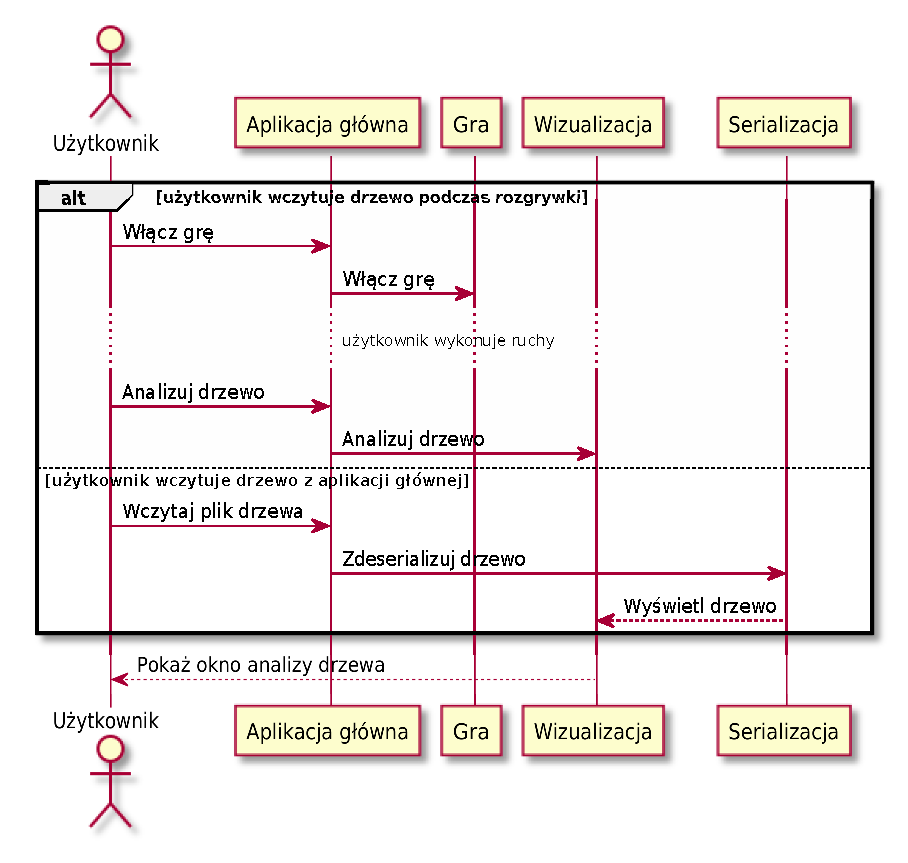
\includegraphics[width=0.7\textwidth]{visualization_sequence_simplified}
	\caption{Diagram sekwencji wizualizacji}
	\label{rys:sequencevisualise}
\end{figure}

\noindent Ważne jest, że użytkownik może uruchomić wizualizację z poziomu rozgrywki tuż po wygenerowaniu nowego drzewa przez algorytm lub już na etapie menu głównego. Gdy żądanie jest z poziomu rozgrywki, komponent \modulename{Aplikacja główna} komunikuje się z komponentem \modulename{Wizualizacja}, który generuje aktualne drzewo i pokazuje je użytkownikowi w nowym oknie. \\

\noindent Drugi sposób (żądanie analizy drzewa z menu głównego) wymaga wcześniejszego wczytania drzewa z pliku i odpowiednio jego deserializację w celu wyświetlenia - wymaga to komunikacji modułu \modulename{Wizualizacja} i \modulename{Serializacja}, gdzie ten drugi będzie zwracał wynik deserializacji temu pierwszemu. Następnie, analogicznie, użytkownik będzie mógł zobaczyć okno z wygenerowanym drzewem.\\

\noindent Interakcja wyżej wymienionych komponentów wygląda tak samo również w przypadku, gdy użytkownik poprosi o przeanalizowanie większej ilości drzew za jednym razem.


\section{Raport z testów akceptacyjnych}
Testy akceptacyjne zostały przeprowadzone w celu sprawdzenia, czy aplikacja spełnia założenia opisane w dokumentacji wymagań projektu. Test \ref{tab:test1} konfrontuje założenia modułu \modulename{Gry}, test \ref{tab:test2} - modułu \modulename{Serializacja}, a pozostałe testy weryfikują założenia modułu \modulename{Wizualizacja}. \\

\noindent Testy akceptacyjne zostały wykonane na komputerze:
\begin{itemize}
	\item z zainstalowanym systemem operacyjnym \modulename{Windows 10 Education N},
	\item z zainstalowanym interpreterem języka \modulename{Python 3.7.2} i biblioteką \modulename{PyQt5},
	\item wyposażonym w procesor \modulename{Intel Core i7-8700k @3.70 GHz},
	\item wyposażonym w kartę graficzną \modulename{NVIDIA GeForce GTX 1060 6GB},
	\item wyposażonym w 32GB pamięci RAM.
\end{itemize}

\begin{table}[h!]
\centering
\begin{tabular}{|l|p{0.6\linewidth}|}
	\hline
	Testowane wymaganie & \modulename{Użytkownik będzie mógł wybrać jedną z dwóch przykładowych gier, a do wyboru będzie miał trzy tryby rozgrywki.} \\ \hline
	Kroki testowe & \begin{enumerate} \item Z menu głównego aplikacji wybierz opcję \modulename{Chess}. \item Z menu głównego aplikacji wybierz opcję \modulename{Player vs player} i sprawdź tryb rozgrywki dla dwóch graczy. \item Z menu głównego aplikacji wybierz opcję \modulename{Player vs PC} dla różnych ustawień algorytmu UCT. \item Z menu głównego aplikacji wybierz opcję \modulename{PC vs PC} dla różnych ustawień algorytmu UCT. \item Z menu głównego aplikacji wybierz \modulename{Mancala} i powtórz kroki 2-5. \end{enumerate} \\ \hline
	Wynik & Pozytywny. \\ \hline
\end{tabular}
\caption{Raport z pierwszego testu}
\label{tab:test1}
\end{table}

\begin{table}[h!]
	\centering
	\begin{tabular}{|l|p{0.6\linewidth}|}
		\hline
		Testowane wymaganie & \modulename{Użytkownik będzie mógł zapisać analizowane drzewa do pliku csv, do pliku binarnego oraz do bitmapy.} \\ \hline
		Kroki testowe & \begin{enumerate} \item Z menu głównego aplikacji wybierz ścieżkę do dowolnego pliku z zserializowanym drzewem. \item Naciśnij przycisk \modulename{Inspect tree}. \item Naciśnij przycisk \modulename{Save to csv file}. \item Naciśnij przycisk \modulename{Save to binary file}. \item Naciśnij przycisk \modulename{Save to bitmap file}. \item Sprawdź, czy bitmapa wygenerowana w kroku 5 odpowiada drzewu z pliku początkowego. \item Z menu głównego aplikacji wybierz ścieżkę plików wygenerowanych w kroku 3 i 4, żeby sprawdzić, czy zapisane drzewa wizualizowane są tak samo jak w początkowym pliku. \end{enumerate} \\ \hline
		Wynik & Pozytywny. \\ \hline
	\end{tabular}
	\caption{Raport z drugiego testu}
	\label{tab:test2}
\end{table}

\clearpage

\begin{table}[h!]
	\centering
	\begin{tabular}{|l|p{0.6\linewidth}|}
		\hline
		Testowane wymaganie & \modulename{Użytkownik będzie mógł wyświetlić informacje związane z wybranym węzłem drzewa, a także przybliżać i oddalać cały graf.} \\ \hline
		Kroki testowe & \begin{enumerate} \item Z menu głównego aplikacji wybierz ścieżkę do dowolnego pliku z drzewem. \item Naciśnij przycisk \modulename{Inspect tree}. \item Przy użyciu prawego przycisku myszki chwyć za obszar rysowania i poruszaj się po wizualizacji. \item Używając kółka myszki, przybliż i oddal wizualizowane drzewo. \item Kliknij dowolny wierzchołek drzewa lewym przyskiem myszki i sprawdź, czy panel z prawej strony wyświetla informacje związane z wybranym wierzchołkiem. \end{enumerate} \\ \hline
		Wynik & Pozytywny. \\ \hline
	\end{tabular}
	\caption{Raport z trzeciego testu}
	\label{tab:test3}
\end{table}

\begin{table}[h!]
	\centering
	\begin{tabular}{|l|p{0.6\linewidth}|}
		\hline
		Testowane wymaganie & \modulename{Dla drzew do 100 000 wierzchołków wizualizacja nie powinna zajmować więcej niż 3s.} \\ \hline
		Kroki testowe & \begin{enumerate} \item Z menu głównego aplikacji wybierz ścieżkę do pliku \modulename{tree\textunderscore 100k.csv}. \item Naciśnij przycisk \modulename{Inspect tree}. \end{enumerate} \\ \hline
		Wynik & Pozytywny - deserializacja, ulepszony algorytm Walkera i wyświetlenie drzewa z pliku zajęło 2.802s. \\ \hline
	\end{tabular}
	\caption{Raport z czwartego testu}
	\label{tab:test4}
\end{table}

\begin{table}[h!]
	\centering
	\begin{tabular}{|l|p{0.6\linewidth}|}
		\hline
		Testowane wymaganie & \modulename{Dla drzew do 250 000 wierzchołków wizualizacja nie powinna zajmować więcej niż 5s.} \\ \hline
		Kroki testowe & \begin{enumerate} \item Z menu głównego aplikacji wybierz ścieżkę do pliku \modulename{tree\textunderscore 250k.csv}. \item Naciśnij przycisk \modulename{Inspect tree}. \end{enumerate} \\ \hline
		Wynik & Pozytywny - deserializacja, ulepszony algorytm Walkera i wyświetlenie drzewa z pliku zajęło 4.626s. \\ \hline
	\end{tabular}
	\caption{Raport z piątego testu}
	\label{tab:test5}
\end{table}

Wszystkie testy akceptacyjne zakończyły się pozytywnie, a więc wymagania zostały spełnione.


\section{Użyte technologie}
W naszym projekcie zdecydowaliśmy się skorzystać z:
\begin{enumerate}
	\item Języka \modulename{Python} w wersji 3.7.2.
	\item Biblioteki \modulename{VisPy} w wersji 0.6.3, która udostępnia komponenty związane z wizualizacją graficzną. Wykorzystujemy tę bibliotekę w połączeniu z \modulename{OpenGL} w wersji 2.1. Biblioteka \modulename{VisPy} jest stworzona w oparciu o licencję \modulename{BSD}, co w kontekście projektu na pracę inżynierską pozwala na modyfikowanie i wykorzystywanie jej.
	\item \modulename{PyQt5} - nakładki na bibliotekę Qt, umożliwiającą tworzenie interfejsu graficznego. Dla projektów takich jak praca inżynierska, \modulename{PyQt} dystrybuowana jest na zasadach \modulename{GNU General Public License}.
\end{enumerate}
\end{document}
